Consider the empirical risk from above. The Hessian matrix w.r.t.\,to a flattening scheme $\vec$ is given by
\begin{align*}
  \hess_{\vtheta}^{\vec} \gL_{\sD}(\vtheta)
  =
  R
  \sum_{n=1}^N
  \hess_{\vtheta}^{\vec} \ell_n(\vtheta) \in \sR^{D \times D}\,.
\end{align*}
and contains the second-order partial derivatives of $\gL_{\sD}(\vtheta)$, that is
\begin{align*}
  [\hess_{\vtheta}^{\vec} \gL_{\sD}(\vtheta)]_{i,j}
  =
  \frac{\partial^2 \gL_{\sD}(\vtheta)}{\partial [\vec(\vtheta)]_i \partial [\vec(\vtheta)]_j}\,.
\end{align*}

\switchcolumn[1]*
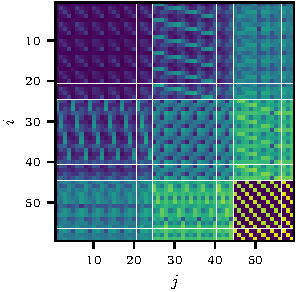
\includegraphics{../kfs/plots/synthetic_cvec_hessian.pdf}

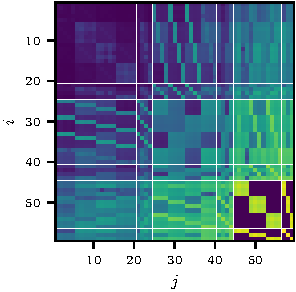
\includegraphics{../kfs/plots/synthetic_rvec_hessian.pdf}
\switchcolumn[0]

Due to the tuple/list structure of $\vtheta$, the Hessian has a block structure,
\begin{align*}
  \hess_{\vtheta}^{\vec} \gL_{\sD}(\vtheta)
  =
  \begin{pmatrix}
    \hess_{\vtheta^{(1)}}^{\vec} \gL_{\sD}(\vtheta)
    &
      \hess_{\vtheta^{(1)}, \vtheta^{(2)}}^{\vec} \gL_{\sD}(\vtheta)
    &
      \cdots
    &
      \hess_{\vtheta^{(1)}, \vtheta^{(L)}}^{\vec} \gL_{\sD}(\vtheta)
    \\
    \hess_{\vtheta^{(2)}, \vtheta^{(1)}}^{\vec} \gL_{\sD}(\vtheta)
    &
      \hess_{\vtheta^{(2)}}^{\vec} \gL_{\sD}(\vtheta)
    &
      \cdots
    &
      \hess_{\vtheta^{(2)}, \vtheta^{(L)}}^{\vec} \gL_{\sD}(\vtheta)
    \\
    \vdots & \cdots & \ddots & \vdots
    \\
    \hess_{\vtheta^{(L)}, \vtheta^{(1)}}^{\vec} \gL_{\sD}(\vtheta)
    &
      \hess_{\vtheta^{(L)}, \vtheta^{(2)}}^{\vec} \gL_{\sD}(\vtheta)
    &
      \cdots
    &
      \hess_{\vtheta^{(L)}}^{\vec} \gL_{\sD}(\vtheta)
  \end{pmatrix}\,.
\end{align*}
where $\hess_{\vtheta^{(i)}, \vtheta^{(j)}}^{\vec} \gL_{\sD}(\vtheta)$ contains mixed second-order partial derivatives w.r.t.\,$\vtheta^{(i)}$ and $\vtheta^{(j)}$.

In the following, we will only consider the block diagonal approximation of this matrix,
\begin{align*}
  \tilde{\hess}_{\vtheta}^{\vec} \gL_{\sD}(\vtheta)
  =
  \begin{pmatrix}
    \hess_{\vtheta^{(1)}}^{\vec} \gL_{\sD}(\vtheta)
    &
      \vzero
    &
      \cdots
    &
      \cdots
    &
      \vzero
    \\
    \vzero
    &
      \hess_{\vtheta^{(2)}}^{\vec} \gL_{\sD}(\vtheta)
    &
      \vzero
    &
      \cdots
    &
      \vzero
    \\
    \vdots & \cdots & \ddots & \vdots
    \\
    \vzero
    &
      \vzero
    &
      \vzero
    &
      \cdots
      &
      \hess_{\vtheta^{(L)}}^{\vec} \gL_{\sD}(\vtheta)
  \end{pmatrix}\,.
\end{align*}
i.e., individual blocks $\{ \hess_{\vtheta^{(i)}}^{\vec} \gL_{\sD}(\vtheta)$.

%%% Local Variables:
%%% mode: latex
%%% TeX-master: "../main"
%%% End:
